\chapter{Literature review}

\section{Trends in humanoid robotics}

The word ``Robot'' first appeared in Karel Capek's 1921 play \textit{Rossum's Universal Robots} where the \textit{robots} were human-like machines made to replace human workers. It comes from the Czech word ``Robota'' which means ``labour doing compulsory manual works without receiving any remuneration'' or ``to make things manually''. Robots are now very widely used in the manufacturing sector. Robotic technology has been developed and refined so successfully that an entire manufacturing process can be handled by robots alone.

The International standard ISO 3873 defines ``Robot'' as: ``An automatically controlled, reprogrammable, multi-purpose, manipulator, programmable in three or more axes, which may be either fixed in place or mobile for use in industrial automation applications''. This definition restricts the area to only one type of robot, the industrial manipulator. But the inclusion of the perception of the environment and a capacity for action with some level of autonomy the robot leaves the manufacturing plant. The continuous evolution of robots needs a more general definition to include other types of robots in the global robotics area. The Oxford dictionary defines ``Robot'' as ``a machine resembling a human being and able to replicate certain human movements and functions automatically''. Nowadays, the robot is leaving factories and laboratories and slowly entering society in the form of a service robot.

\subsection{General classification of robots}
The development of robotics through the ages, makes necessary to do a classification. Based on their ability to make different types of motion, their control architectures differ radically. Five groups of robotic systems can be distinguished by their motion control architecture: industrial, mobile, zoomorphic, anthropomorphic and hybrid robots.

\textit{Industrial robots}. The main characteristic of this group is that all robots are stationary. Industrial robots, including industrial manipulators (Figure \ref{fig:abb}) , are usually designed taking into account different requirements for velocity, load capacity, accessibility, etc. and always have different number of degrees of freedom. These robots are structured to move their end effectors in a determined working environment in one or several systems of coordinates. Although, exceptions may exist when a robot is guided in space (with moving platform) in order to perform a task in another environment. These robots are used when it is necessary to attend rather extensive but permanent working zones, working mainly with different types of objects and environments and does not exist human-robot interaction.
\begin{figure}[!hbt]
\centering
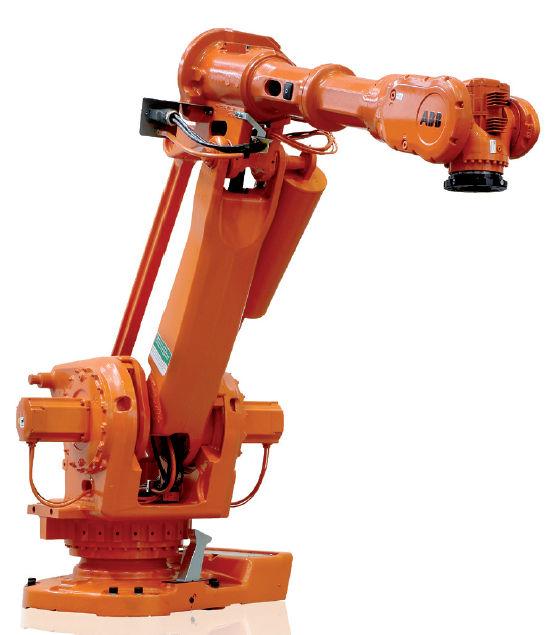
\includegraphics[scale=0.35]{abb.jpg}
\caption{ABB industrial manipulator}
\label{fig:abb}
\end{figure}
 
\textit{Mobile robots}. This group has more motion capacity due to implemented wheel based platform systems (Figure \ref{fig:mobile}). They can execute different telecontrolled tasks or are driven by the environmental information received from the integrated sensorial system. The motorized turtle designed in 1948 by Walter was the first predecessor. From the beginning of the sixties mobile robots were designed and implemented within industry. These robots were able to transport parts from one point of the production line to another, guided by preplanned paths materialized by the electromagnetic or photoelectric bands from circuits mounted into the floor. From the beginning of the seventies a lot of work was related to major autonomy of mobile robots. It involved providing the mobile robot with a vision system \textcolor{red}{[Moravec, 1981]}. Finally, from the beginning of the eighties, when more complex and precise sensorial systems appeared, the development of architectures for control of mobile robots was concentrated on the superficial intelligence and decision making systems \textcolor{red}{[Bares, 1998], [Thorpe, 1990]}. Mobile robots provided with this kind of control system are usually able to plan motions and avoid obstacles. Today, research is also centred on human-mobile robot interaction \textcolor{red}{[Khamis 2007]}. 

\begin{figure}[!hbt]
\centering
\subfigure[TurtleBot mobile robot]{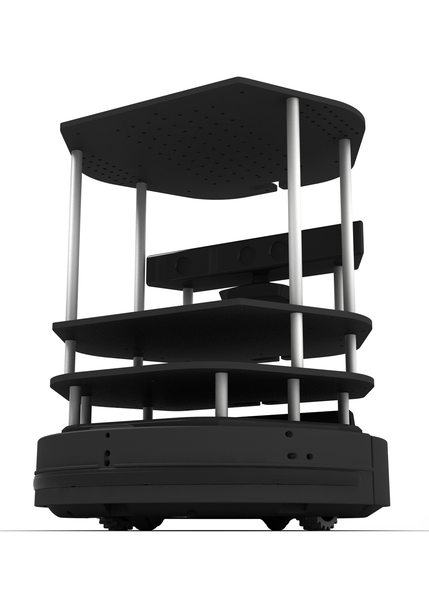
\includegraphics[width=30mm]{turtlebot.png}}\hspace{10mm}
\subfigure[MAGGIE social robot from UC3M]{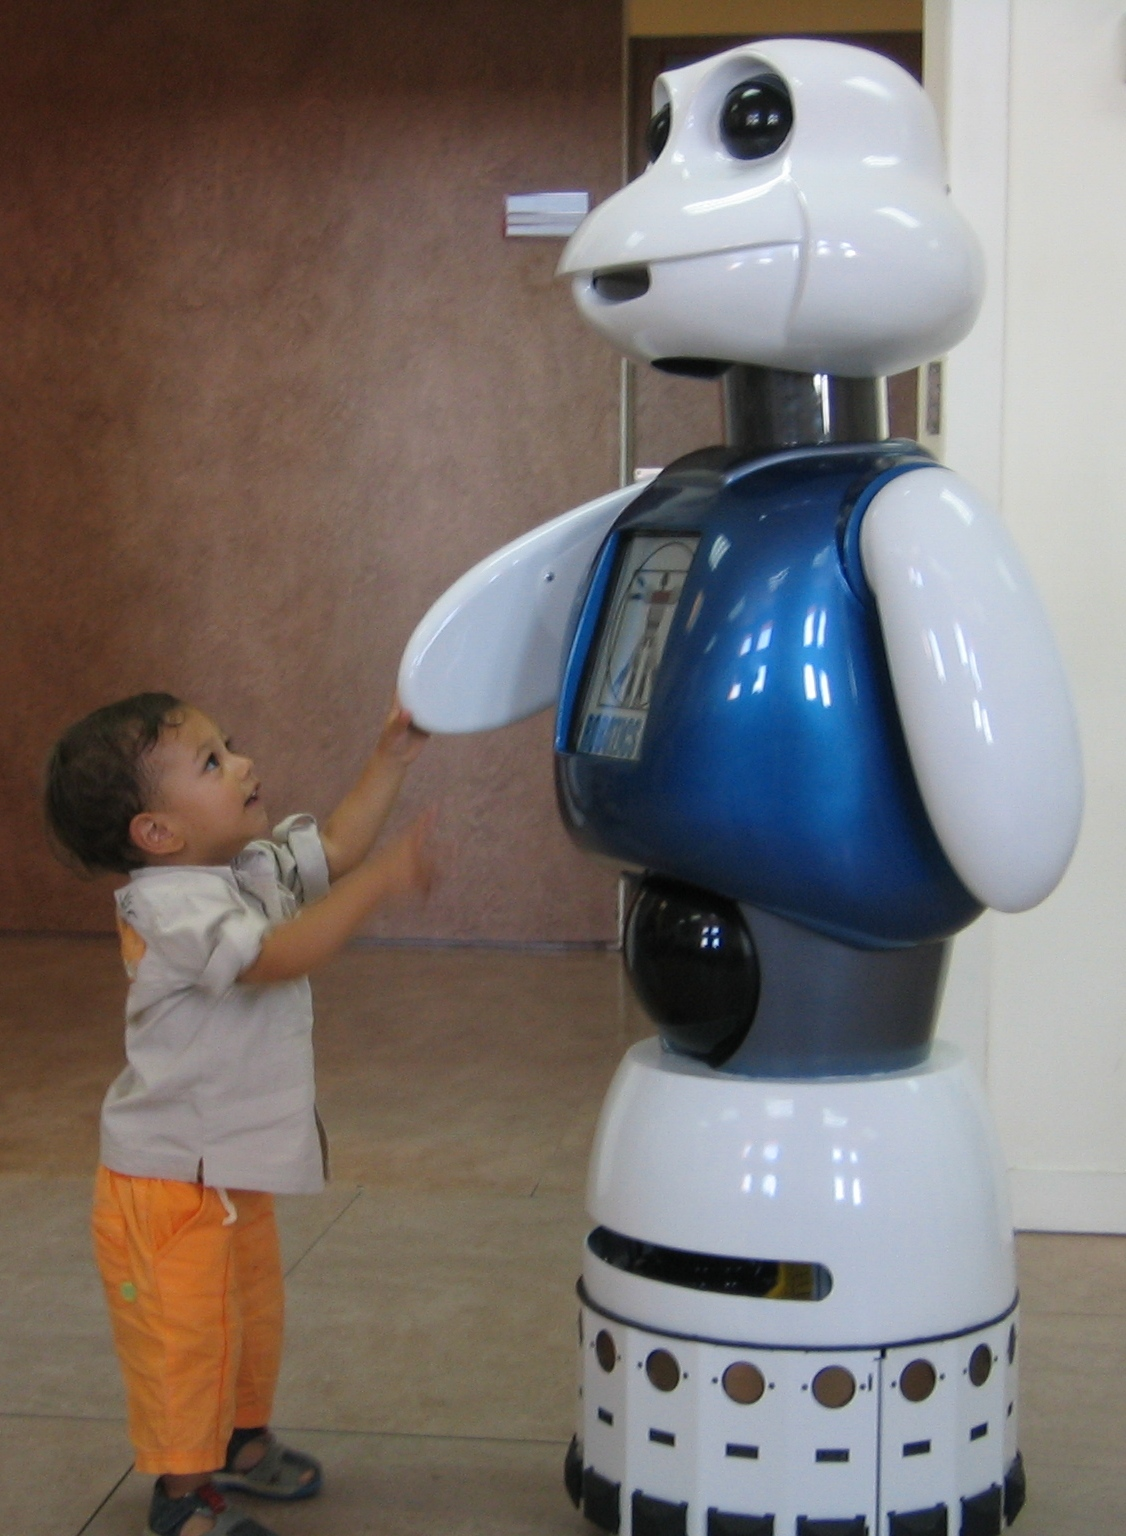
\includegraphics[width=30mm]{maggie.jpg}}
\caption{Mobile robots}
\label{fig:mobile}
\end{figure}

\textit{Zoomorphic robots}. This type of robot is characterized by the locomotion system which imitates the locomotion of diverse living beings. Although there can be a lot of morphological differences between all variations of zoomorphic systems, it is possible to distinguish two basic categories: walking and non-walking zoomorphic architectures. An example of non-walking zoomorphic robot is the modular snake-like robot in Figure \ref{fig:zoo} (a). Walking zoomorphic robots are developed to work in every king of terrain and they have a really wide range of applications. It could be spatial research, out-of-the-way terrain exploration, or volcanic research. Animal-like robots try to imitate the movements of animals and are usually constructed for research and entertainment. The control of this kind of robot is more complicated than control of a mobile or polyarticulated robot because of the need to maintain the equilibrium at every stage of motion. Figure \ref{fig:zoo} (b) shows the WildCat walking zoomorphic robot developed by Boston Dynamics.

\begin{figure}[!hbt]
\centering 
\subfigure[Non-walking zoomorphic robot]{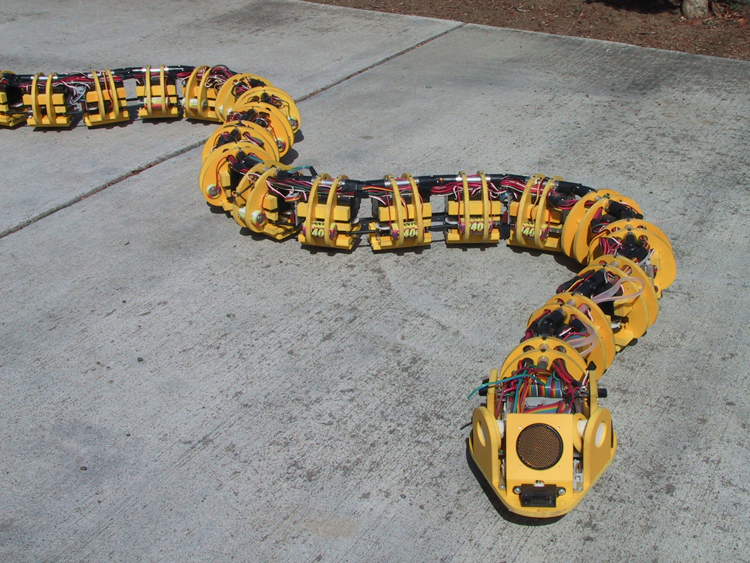
\includegraphics[width=40mm]{snake.jpg}}\hspace{10mm}
\subfigure[WildCat walking zoomporphic robot]{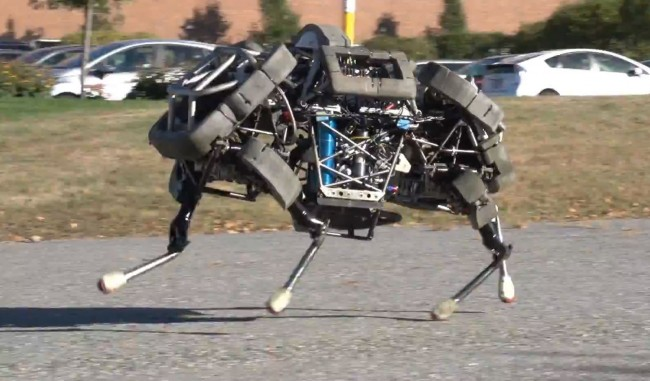
\includegraphics[width=40mm]{wildcat.jpg}}
\caption{Zoomporphic robots}
\label{fig:zoo}
\end{figure}

\textit{Anthropomorphic robots (Androids)} or humanoid (bipedal) robots. These robots try to reproduce the body and behaviours of a human being. Presently the research on humanoids is increasing rapidly, although, there still remains a lot of work ahead. One of the basic challenges in this field is to reproduce human-like motion abilities beginning with the bipedal locomotion \textcolor{red}{[Hirai 98]}. The motion control architecture in this case is the most complex compared with the other robot types presented above. The main challenge is being able to control and coordinate in real time the dynamics of the entire body and maintain the equilibrium in the single support phase, i.e. when the robot is supported only by one foot. The control architecture of this kind of robot is an aim of the presented research and will be discussed and developed further in the following chapters. Figure \ref{fig:humanoid} shows two examples of humanoid robots: (a) is Asimo Robot developed by Honda and (b) is TEO robot from UC3M.

\begin{figure}[!hbt]
\centering 
\subfigure[ASIMO robot]{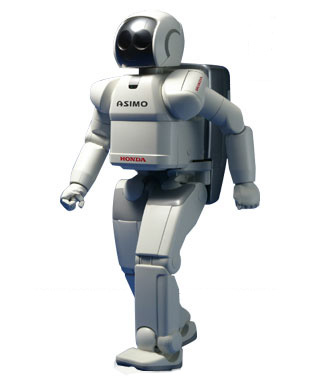
\includegraphics[width=30mm]{asimo.jpg}}\hspace{10mm}
\subfigure[TEO robot]{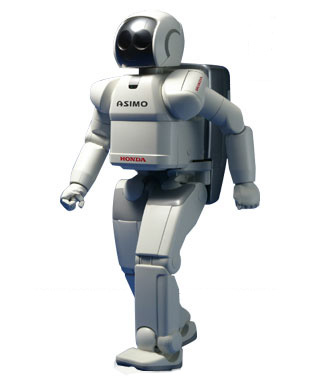
\includegraphics[width=30mm]{asimo.jpg}}
\caption{Humanoid robots}
\label{fig:zoo}
\end{figure}


Another complex aspect related to androids is the ability to reproduce the human upper body, especially the face. The difference between a humanoid robot and android is only skin-deep. The latter looks exactly like a human on the outside, but internally has the mechanics of a humanoid robot. But the human-like appearance can be controversial. In 1970, Masahiro Mori presented his hypothesis about the \textit{Uncanny Valley} (Figure \ref{fig:valley}). Mori's insight was that people would react with revulsion to human-like robots, whose appearance resembled, but did not quite replicate, that of a real human. The Uncanny Valley has become more relevant in the past few years since robots that actually look and move like humans are starting to become a reality. In fact, researchers currently debate over whether they should try to overcome the uncanny valley or simply design robots that are more mechanical in appearance.

\begin{figure}[!hbt]
\centering
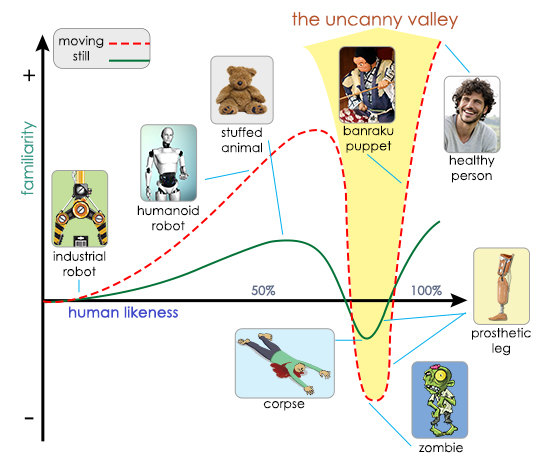
\includegraphics[scale=0.45]{valley.jpg}
\caption{Uncanny valley}
\label{fig:valley}
\end{figure}


\textit{Hybrid robots.} These type  of robots combine properties of various types of other robots. Usually they are a combination of a wheelbase (mobile robot) with an anthropomorphic body. Some examples are Justin robot from the German Aerospace Center (DLR) and TIAGO robot from PAL Robotics (Figure \ref{fig:hybrid}). They are both mainly involved in manipulation tasks (grasping, picking and placing, etc.) and the problem of locomotion in not considered as in humanoids. 

\begin{figure}[!hbt]
\centering 
\subfigure[Justin robot]{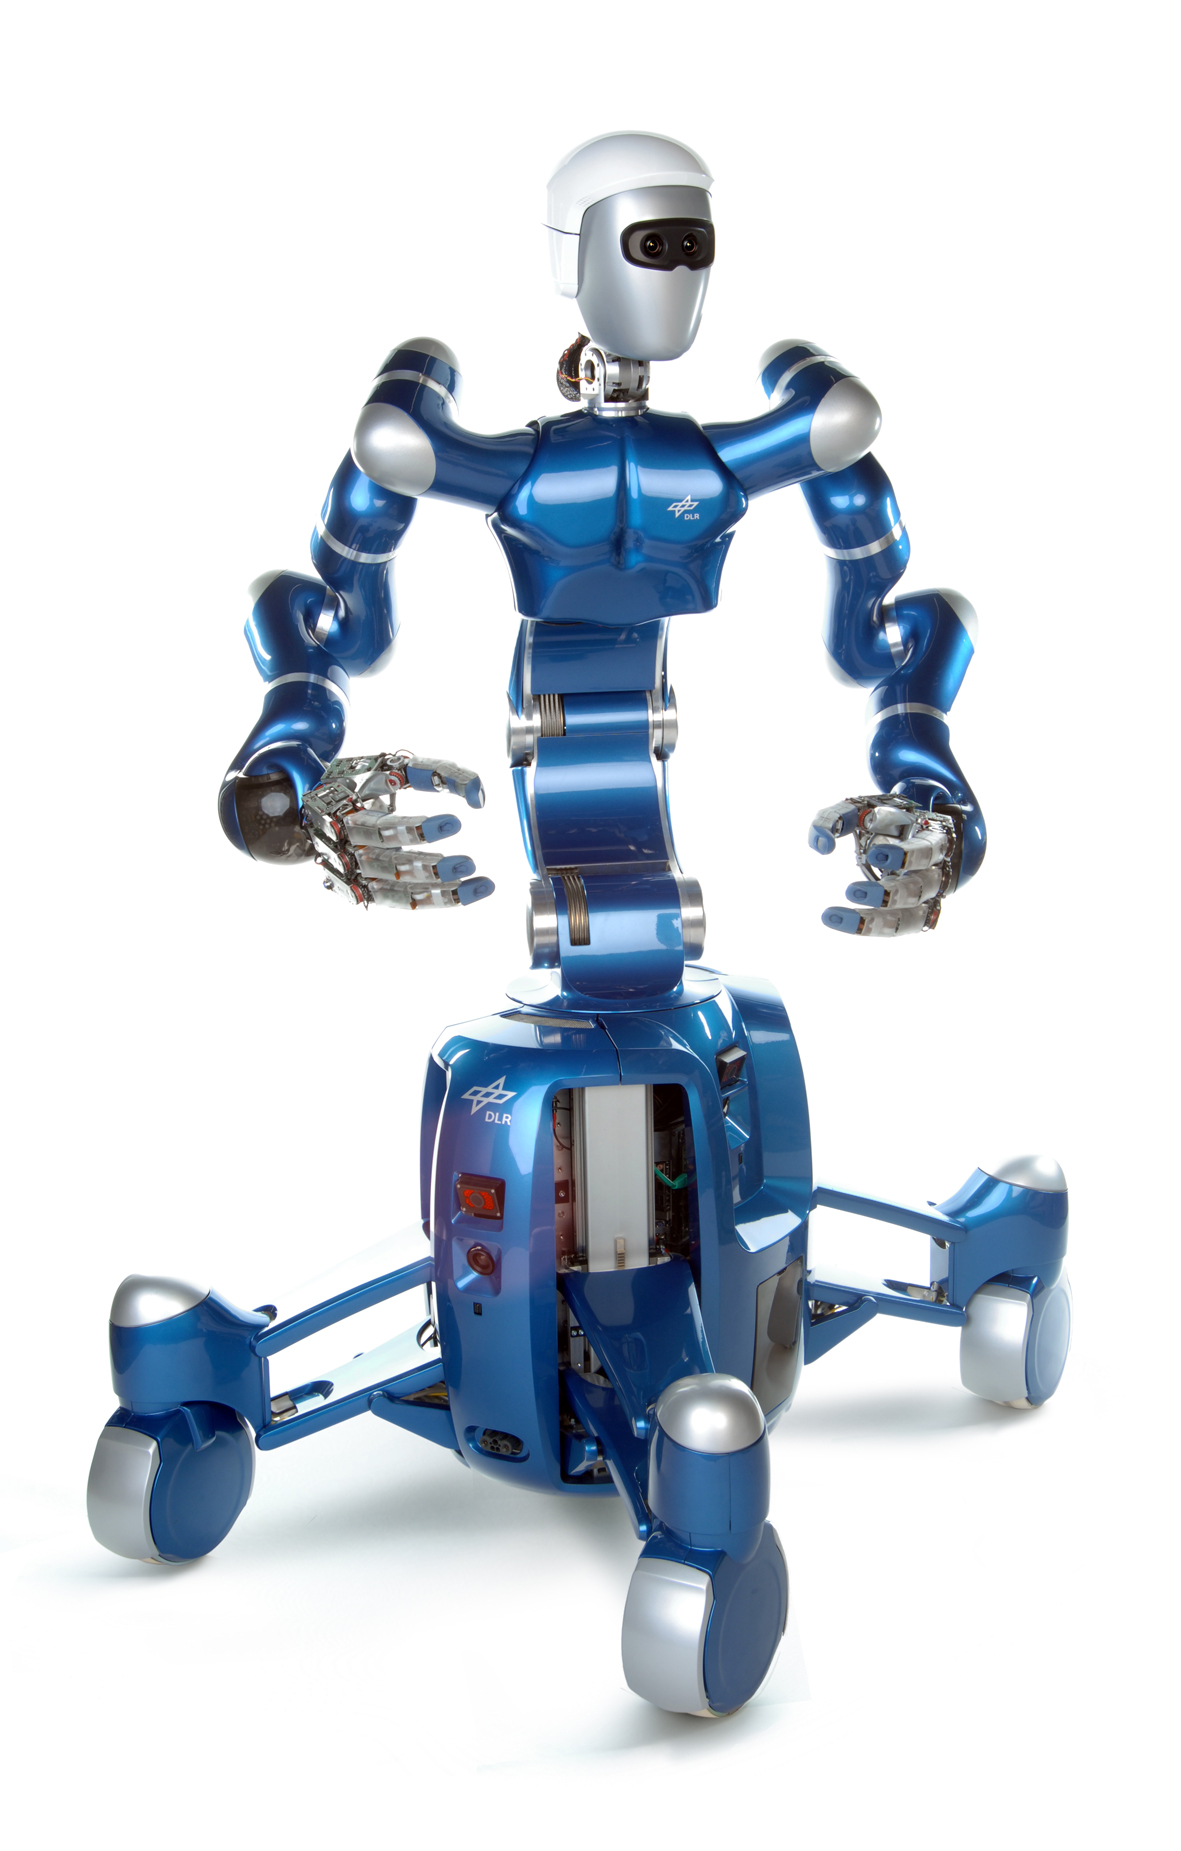
\includegraphics[width=30mm]{justin.jpg}}\hspace{10mm}
\subfigure[TIAGO robot]{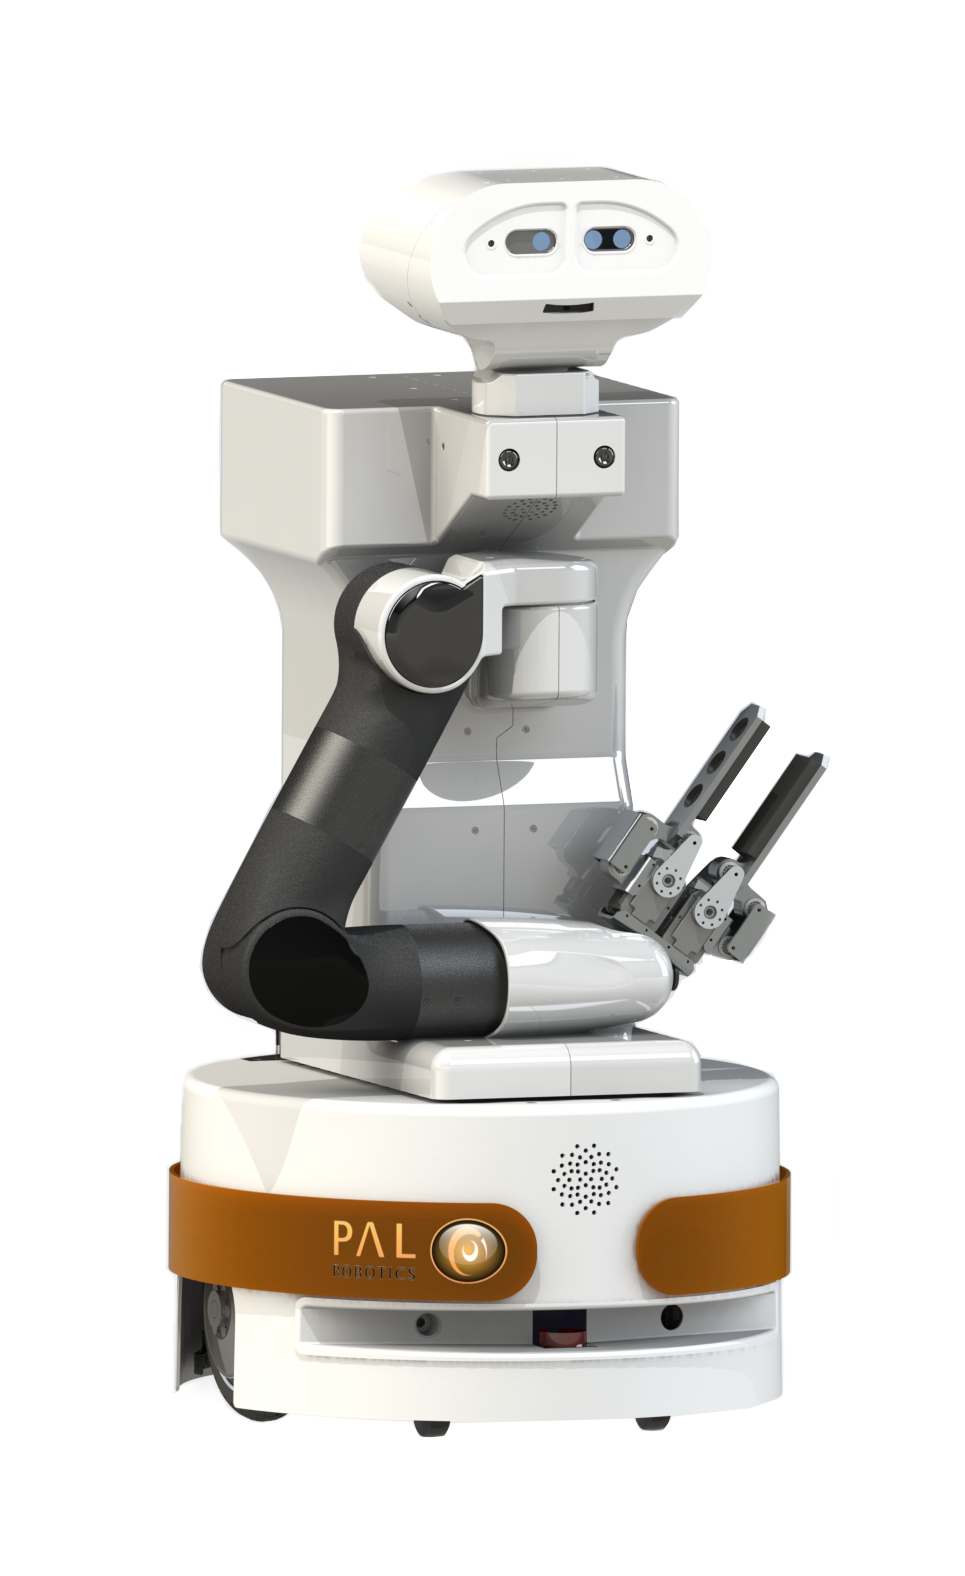
\includegraphics[width=30mm]{tiago.jpg}}
\caption{Hybrid robots}
\label{fig:hybrid}
\end{figure}

\newpage



\subsection{Humanoid robots}

The history of the development of humanoid robots is curiously long and detailed. Leonardo da Vinci designed and possibly built the first humanoid robot (\ref{fig:knight}). The robot, completely mechanical, was designed to sit up, wave arms and move its head via a flexible neck while opening and closing its jaw. 

\begin{figure}[!hbt]
\centering
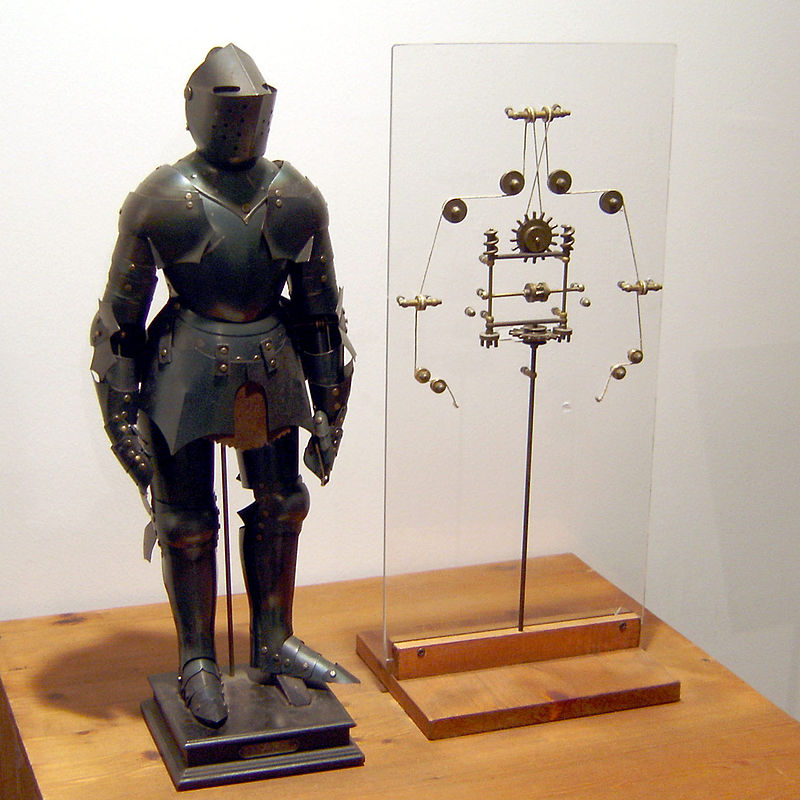
\includegraphics[scale=0.15]{knight.jpg}
\caption{Leonardo da Vinci's mechanical knight}
\label{fig:knight}
\end{figure}

Other designs, related to the appearance of steam power and electricity appeared in the 19\up{th} Century. They were simple automates that imitated some human movements. The first bipedal machine was constructed by George Moore in 1983 but the real progress was achieved only at the end of the 1960s when the electronics, mechanics and materials became sufficiently advance to create such a complex system as a bipedal robot.

In the middle of the 1960s, the Japan University of Waseda launched different research projects lead by Kato and as a result, the series of WL robots appeared. They were only lower body robots (Figure \ref{fig:wl}).

\begin{figure}[!hbt]
\centering 
\subfigure[]{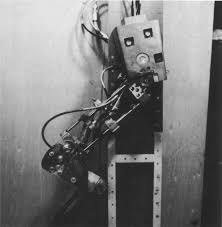
\includegraphics[width=40mm]{wl1.jpeg}}\hspace{10mm}
\subfigure[]{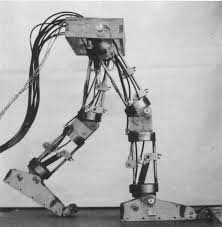
\includegraphics[width=40mm]{wl3.jpeg}}
\caption{(a) WL-1 (b)WL-3}
\label{fig:wl}
\end{figure}

But the real first works about bipedal robots with humanoid appearance (complete torso) were carried out about 1970 by authors Kato \cite{Kaj2005} and Vukobratović \ref{Vuk1970}. The first anthropomorphic robot WABOT-1 (Figure \ref{fig:wabot}), was exhibited by Kato in 1973. Using a very simple control diagram, the robot was able to perform a few slow gaits, maintaining its balance at all times. This achievement, was the first one that encouraged researchers about humanoid robots and their locomotion.

At the same time, Vukobratović and his research team were studying stability in biped systems in the former Yugoslavia, basing on a new stability criterion, presented in 1972, as \textit{Zero-Moment Point (ZMP)}. Taking into account the dynamic effects produced during a walking, from then until now, the ZMP stability criterion has been the most used in humanoid or biped robotics.

The second prototype WABOT-2 of Waseda University was developed between 1980 and 1984. The robot musician WABOT-2 can converse with a person, read a normal musical score with its eyes and play tunes on an electronic piano. The WABOT-2 can be mentioned as one of the first personal robots.

\begin{figure}[!hbt]
\centering 
\subfigure[]{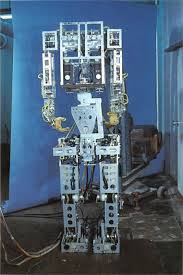
\includegraphics[width=40mm,height=50mm,keepaspectratio]{wabot1.jpeg}}\hspace{10mm}
\subfigure[]{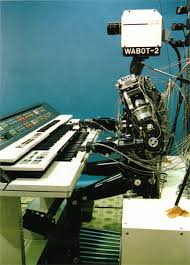
\includegraphics[width=40mm,height=50mm,keepaspectratio]{wabot2.jpeg}}
\caption{(a) WABOT-1 (b)WABOT-2}
\label{fig:wabot}
\end{figure}

Years later, the proyect continued in the Japanese university and the WABIAN series (Figure \ref{fig:wabian}) were constructed as improvements of the previous ones. These robots had advances in their degrees of freedom, better mechanical structure, better stability and bigger weight of objects to be transported. The WABIAN series is still in development with its latest prototype WABIAN 2-R. New technologies and materials make a huge difference between this and the first versions. An important advantage of its mechanical design is the use of 2-DOF in the waist which enables more fluent walking motions. 

\begin{figure}[!hbt]
\centering 
\subfigure[]{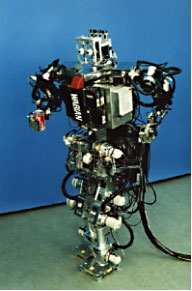
\includegraphics[width=30mm,height=40mm,keepaspectratio]{wabian.JPG}}\hspace{10mm}
\subfigure[]{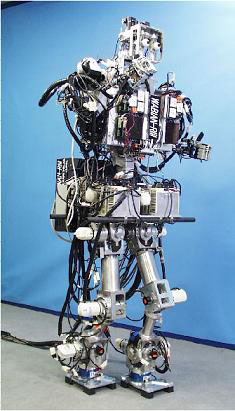
\includegraphics[width=30mm,height=40mm,keepaspectratio]{wabianrv.JPG}}
\hspace{10mm}
\subfigure[]{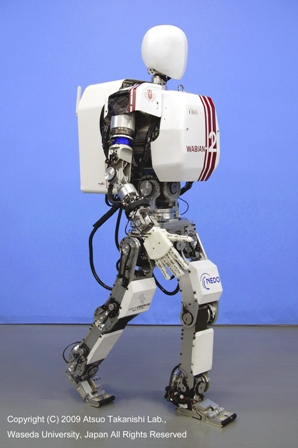
\includegraphics[width=30mm,height=40mm,keepaspectratio]{wabian2r.jpg}}
\caption{(a) WABIAN (b) WABIAN-RV (c) WABIAN-2R }
\label{fig:wabian}
\end{figure}

The development of humanoid robotics was not only at universities also in industry. The Honda Motor Company was one of the main pathfinder industries involved in robotics. In the mid 1980s, they began creating biped walking robots (only lower body parts). But the rise of humanoid robots started with the development of P1 robot in 1993 \cite{Kaj2005}. The project began in secret years before, after the exhibition of WABOT-2 playing the piano. The next version, P2 in 1996 (180 centimetres high and 210 kg weight), was the first humanoid able to walk in a stable enough way and carry its processor and battery on its back. After that, robots P3 and ASIMO were its advanced versions, reducing hight and weight of the robot.


\begin{figure}[!hbt]
\centering
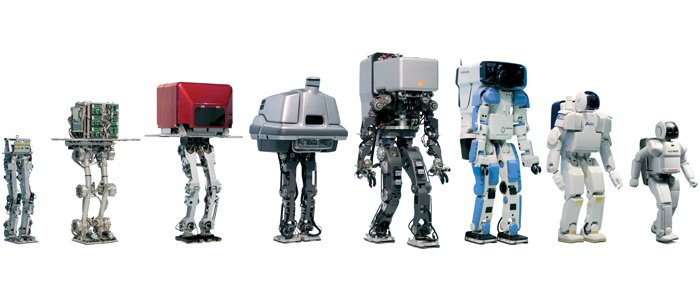
\includegraphics[scale=0.5]{honda.jpg}
\caption{Honda humanoid prototypes. From left to right: E0 (1986) , E1(1987), E3(1989), E5(1992), P1(1993), P2(1996), P3(1997), ASIMO(2000)}
\label{fig:knight}
\end{figure}

Undoubtedly, ASIMO is the culmination of two decades of research in humnaoid robotics by Honda. ASIMO (130 centimetres and 54 kg) is able to run, walk on uneven and slope surfaces, climb stairs, grasp objects among other tasks. It also can avoid moving obstacles as it moves through its environment. 







\section{Bipedal locomotion}
Artificial bipedal locomotion is a complex task and humans have the ideal locomotion. Therefore the best way to reproduce a type of motion for a walking machine is to copy human motion.

Human walking is an automated motion, carried out even uncounciously. This locomotion process is a repetitive execution until some perturbations are detected. In humans, the muscular system modifies forces acting during the walk in order to maintain balance. The study of human wakling and the muscles involved in, brings very complex relationships and it requires some simplifications in anthropomorphic legged mechanisms in order to reduce complexity form the mechanical and control points of view.

The analysis of the human walking is fairly recent. McGeer \cite{McGeer1990} built a passive walker in 1990 and showed that his two-legged walker could reproduce stable gait without any controls. However, the most progress was revealed in the active bipedal locomotion \cite{Hirai1998}, \cite{Kaneko2004}, \cite{Park2007}. This type of locomotion is developed and implemented as artificial human-like bipedal motion based on the previous planning of each step and the real-time automatic control of its execution. 

Generally, the study of the human body is based in three basic planes: sagittal, transversal and frontal (Figure \ref{fig:axes}). It is important to mention that the most important motions related to locomotion occur in the sagittal plane because it coincides with the main walking direction. However, the combination of joints of sagittal and frontal planes, give the stability of the locomotion cycle.

\begin{figure}[!h]
\centering
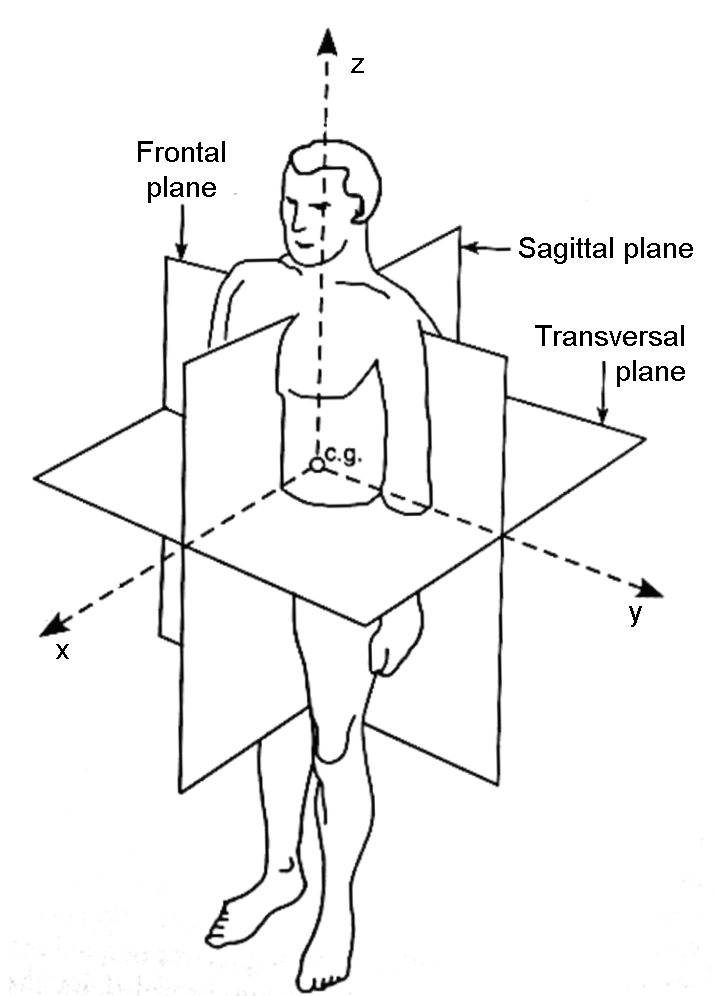
\includegraphics[scale=0.45]{axes.png}
\caption{Axes division of human body.}
\label{fig:axes}
\end{figure}

The basic characteristic of bipedal locomotion is the permanent change of the situation when the mechanism is supported by one foot (single support phase) and when both feet are in contact with the ground (double support phase). The second situation is statically stable and there are no additional moments affecting the robot. In terms of balance, the first situation is statically unstable because when one foot is on the ground, the other is transferred from the back to the front position producing lateral accelerations affecting the mechanism and all the weight remains in only one support foot. Each of these two cases present different dynamical situations and should be taken into account in artificial gait synthesis and control.

Robot walking, as humans, is performed in a three phase cycle (Figure \ref{fig:caminata}). The cycle is divided in two, left and right steps. At the begining, the human is in a stable position with both feet on the ground (Figure \ref{fig:caminata} (a)) and all the body weight is transferred form one foot to the other. Then the step generation starts when the right foot leaves the ground in the swinging phase (Figure \ref{fig:caminata} (b) - (d)). After the right foot touches the ground (Figure \ref{fig:caminata} (e)), the next (left) step with the same basic phases is started, and the whole cycle ends.

Swinging phase has also three sub-phases: acceleration, swinging and deceleration (Figure \ref{fig:caminata} (b), (c) and (d), respectively). The acceleration phase takes its name due to the acceleration of the lifting leg that stops being supported in the ground and gives the impulse to the step. Once the support leg is overtaken, the lifting leg starts the swinging pahse in order to reach the ground with its consequent deceleration.

\begin{figure}[!hbt]
\centering
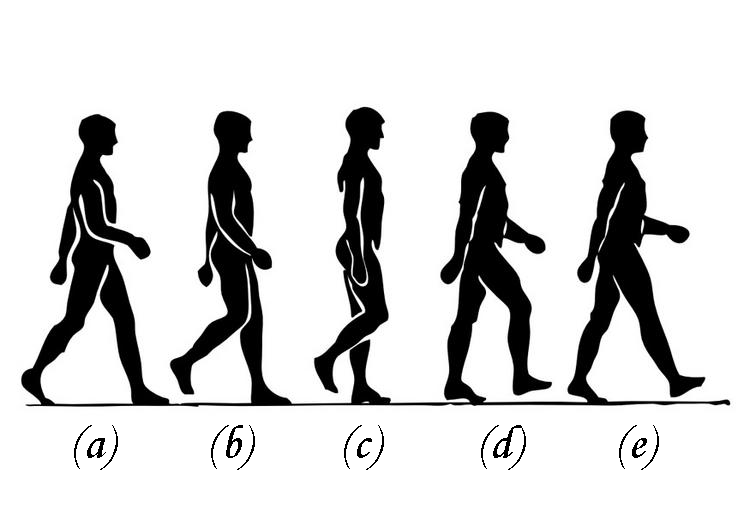
\includegraphics[scale=0.3]{Caminata}
\caption{Phases of biped walking.}
\label{fig:caminata}
\end{figure}

As in the case of the legs, the same occurs with the feet, what adds complexity to control the walking cycle. During a gait, a human foot has four different phases as one can see in Figure \ref{fig:caminata_pie}. In (a) it is shown how the body weight is supported when the heel is touching the ground. In (b), the foot remains totally plane. In (c), the heel lifts and the weight goes to the front part of the foot. Finally, in (d) the foot is not in contact with the ground and it starts to swing.

\begin{figure}[!hbt]
\centering
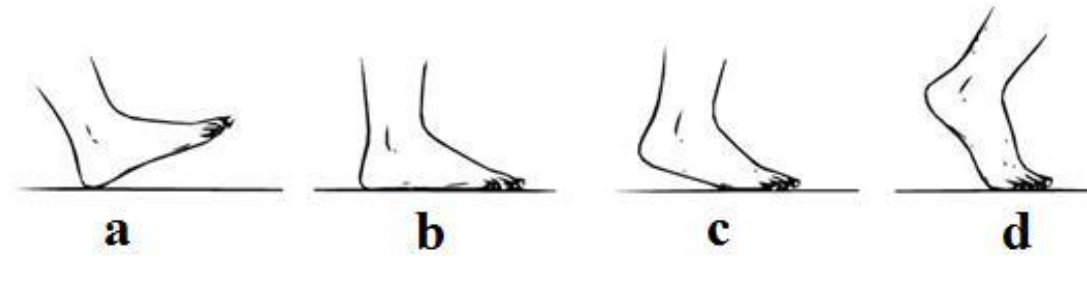
\includegraphics[scale=0.3]{caminata_pie.png}
\caption{Phases of foot support during a walk.}
\label{fig:caminata_pie}
\end{figure}

Almost all humanoid robots do not have articulated feet, due to the high complexity. They use plane and rigid feet and the control is done in the ankle joint. Some of them, as robot HRP-4c \cite{Kan2011}, have a joint called "active toe joint" which allows the movement of the toes. The reason of this improvement is related to reach a more natural and fluent walking.

However, in order to perform a stable walk, is not only necessary the lower body movement. The upper body is also involved in recovery movements. In an example, if a person stumbles. Unwittingly, he or she would move the opposite arm of the unbalanced leg, or even more, moving the torso in order to not to fall down. In the case of a biped robot, the same strategy is followed, what means a high increase of complexity in the robot stability control.

\section{Biped balance/equilibrium}
It is important for humanoid locomotion to avoid overturning during the walking or even to reach an upright position of its body. To prevent falling down, a necessary and suficient condicion is to ensure that there exists a contact area between the foot and the ground and not a line or a point \cite{Vuk2007}. Given a rectangular-shaped foot, the support area of the robot will be a polygon. In case that only on foot is touching the ground (single-support), the support area is the contact region between the sole and the ground, i.e., the footprint (Figure 2.3(a)). On the contrary, when both feet are touching the ground (double-support), the support area will be determined by the footprints and the common tangents between them (Figure 2.3(b)). It means that in double-support phase of the walk, the support area is bigger than in single-support phase, so stability is higher.

\begin{figure}[!hbt]
\centering
\subfigure[Single-support]{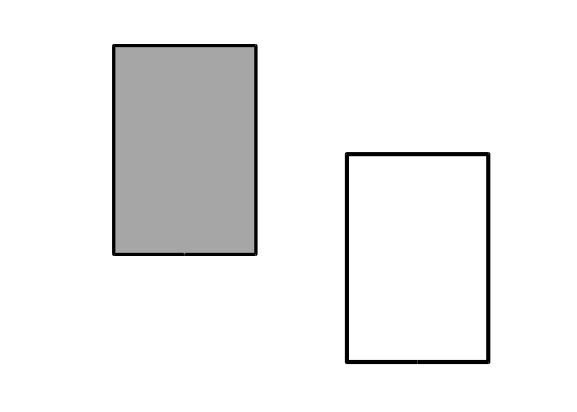
\includegraphics[scale=0.3]{apoyo_simple.png}}
\hspace{10mm}
\subfigure[Double-support]{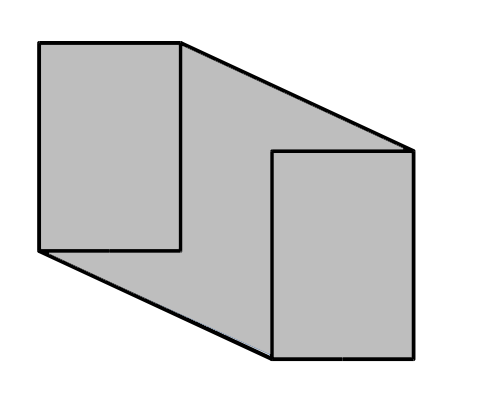
\includegraphics[scale=0.3]{apoyo_doble.png}}
\caption{Support areas depending on the support type.}
\label{fig:apoyo}
\end{figure}


\section{Zero Moment Point (ZMP)}
In \cite{Vuk2007}, Vukobratović makes a distinction between the term ``balance" used in the sense of maintaining an upright posture, and ``equilibrium", taking into account the D'Alembert's principle. The D'Alembert's principle states that the resultant of the external forces and the kinetic reaction acting on a body equals zero (condition of kinetic equilibrium). When the humanoid is falling since it is rotating about one foot edge, the D’Alembert’s principle still holds for a point on the foot edge where the pressure force acts. Anyway, this case cannot be contemplated as balanced in the sense of the definition previously provided. This point is called \textit{Center of Pressure (CoP)} and it is known as the point, in a single-support phase, where the pressure forces (normal to the sole) are equivalent to a single resultant force exerted at the point where the resultant moment is zero.

From the concept of the CoP, appears a new term known as \textit{Zero-Moment Point (ZMP)}. The ZMP is a point inside the support area where, always, the resulting dynamic reaction of the biped system is acting. In a more specific definition, the ZMP is a point inside the support area where the resultant of all forces and torques acting on the full body, is equal to zero.

Vukobratović \cite{Vuk2007} explains the difference between the CoP and ZMP: CoP and ZMP coincide only when both are inside the support area. When the ZMP goes to the edge of the support area, the humanoid body looses balance and it will fall down. In that case, the ZMP has no sense existing even the CoP.

Goswami presented that, mathematically, was possible that the point could be outside of the support area and continue satisfying the equilibrium conditions \cite{Gos}. This point, called \textit{Foot Rotation Indicator (FRI)}, is defined as the point on the contact area between the ground and the foot, inside or outside the suppor area, where the resultant moment of the forces and torques applied on the foot are normal to the surface. Forces and torques applied mean the forces and torques at the ankle joint, and also other external forces, the foot wheight and reaction forces between the foot and the ground. 

However, Vukobratović, held that the ZMP can only exist inside the support area of the robot. When the ZMP comes close to the edge, any force or moment applied to the system, will produce a rotation about the foot edge and the robot will fall down. In this case, the reaction force of the ground will be at the foot edge and, therefore, it can not be considered as ZMP because there is no stability ensured. That is why the author suggests to denote the point as \textit{Fictitious ZMP} o \textit{FZMP}, if it is outside the support area. 
 
When the robot walking is enough slow to consider almost static, appears the term \textit{pseudo-ZMP}, which is the projection over the ground of the \textit{Center of Gravity (CoG)} of the system. In such case, lateral accerlerations are so small and can be omitted and the \textit{pseudo-ZMP} = ZMP. Although the \textit{pseudo-ZMP} do not give precise information about the balance of the mecanism, it can be used in order to make a first aproximation in control and design of a humanoid robot.



\subsection{Equations of ZMP}
Let us consider the locomotion mechanism in the single-support phase, with the whole foot in contact with the ground (Figure \ref{fig:pie} (a)). To simplify the analysis we can neglect the part of the mechanism above the ankle of the support foot (point A) and replace its influence by the force $F_A$ and moment $M_A$, whereby the weight of the foot itself acts at its gravity center (point G). The foot also experiences the ground reaction at point P, whose action keeps the whole mechanism in equilibrium.

\begin{figure}[!hbt]
\centering
\subfigure[]{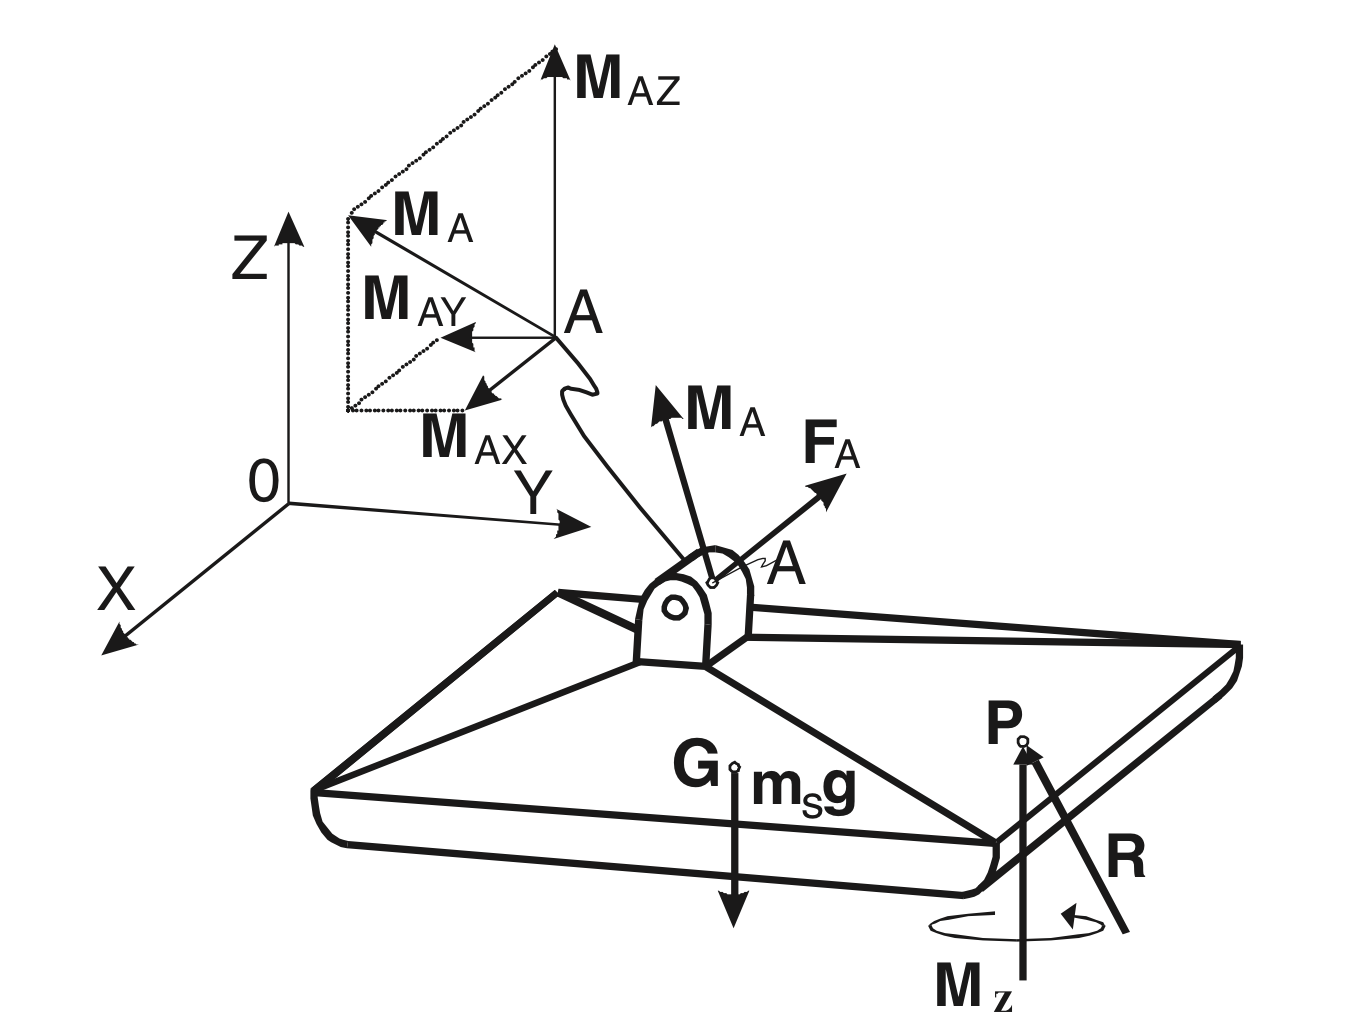
\includegraphics[scale=0.4]{pie.png}}
\subfigure[]{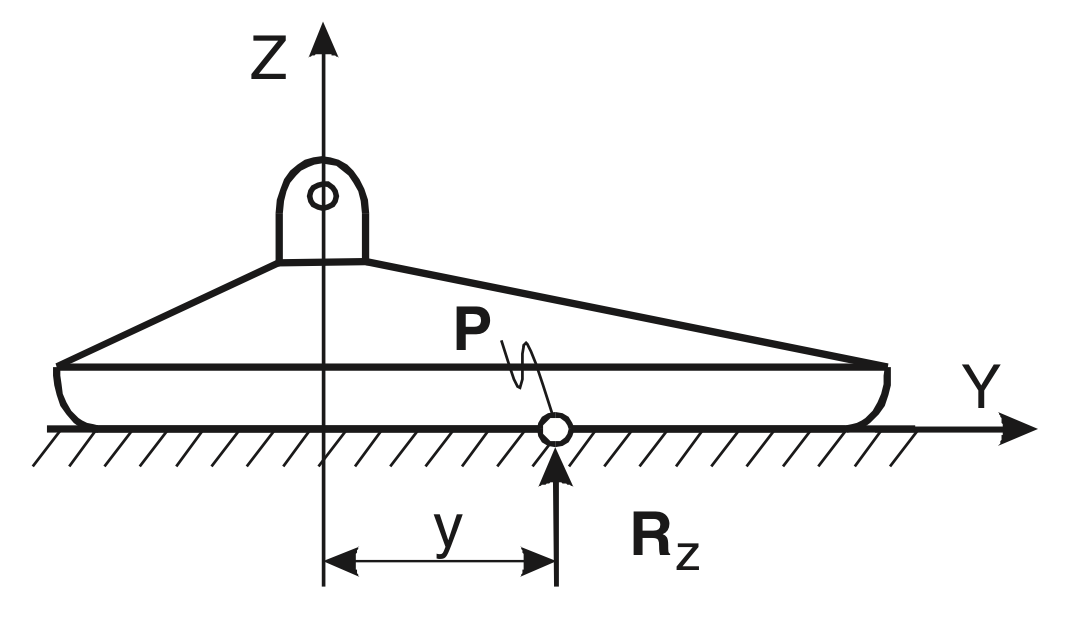
\includegraphics[scale=0.4]{pieYOZ.png}}
\caption{Forces acting on the foot of the bipedal mecanism \protect\cite{Vuk2004} }
\label{fig:pie}
\end{figure}

In general, the total ground reaction consists of three components of the force $R (R_x, R_y, R_z)$ and moment $M (M_x, M_y, M_z)$ exerted at the foot-ground contact point. During the support phase, it is assumed there is no shifting in the contact point, which means that horizontal reaction force $R_x$ and $R_y$ balances the horizontal component of the force $F_A$, whereas the vertical reaction moment $M_z$ represents the moment of friction reaction forces that balances the vertical component of the moment $M_A$ and the moment induced by the force $F_A$.

However, due to an unidirectional nature of the connection between the foot and the ground (it is obvious that the ground reaction force induced by foot action is always oriented upwards) horizontal components of all active moments ($M_A$) can be compensated for only by changing position of the reaction force $R$ within the support polygon. This is illustrated in Figure \ref{fig:pie} (b) where a planar case in $y-z$ plane is represented.

The moment $M_{Ax}$ is balanced by shifting the acting point of the force $R_z$, whose intensity is determined from the equation of balance of all the forces acting on the foot, by the corresponding distance $y$. It is necessary to emphasize that all the time the reaction force is within the area covered by the foot, the increase in the ankle moment will be compensated for by changing the position of this force $R_z$, and no horizontal components of the moments $M_x$ and $M_z$ will exist. This is the reason why in Figure \ref{fig:pie} at point $P$ only the $M_z$ component exists.

However, if the real support polygon is not large enough to encompass the appropriate position of the force $R$ to balance the action of external moments, the force $R$ will act at the foot edge and the uncompensated part of the horizontal component of the reaction moment will cause the mechanism’s rotation about the foot edge, which can result in the mechanism’s overturning. Therefore, it can said that the necessary and sufficient condition for the locomotion mechanism to be in dynamic equilibrium is that for the point $P$ on the sole where the ground reaction force is acting,

\begin{align}
M_x = 0, \nonumber \\
M_y = 0.
\end{align}

That is why the \textit{Zero-Moment Point} is called the contact point with the ground ($P$) where there no exist shifting, i.e., moments $M_x$ y $M_y$ are zero.

From Figure \ref{fig:pie}, static equilibrium equations for the supporting foot are obtained:
\begin{equation}
\sum \overrightarrow{F} = 0 \Rightarrow \overrightarrow{R} + \overrightarrow{F_A} + m_s g = 0
\label{eq:fuerzas}
\end{equation}
\begin{equation}
\sum \overrightarrow{M_O} = 0 \Rightarrow \overrightarrow{OP} \times \overrightarrow{R} + \overrightarrow{OG} \times m_sg + M_A + M_z + \overrightarrow{OA} \times F_A = 0,
\label{eq:momentos}
\end{equation}

where $\overrightarrow{OP}$, $\overrightarrow{OG}$ and $\overrightarrow{OA}$ are radius vectors from the origin of the coordinate system $O_{xyz}$ to the ground reaction force acting point ($P$), foot mass center ($G$), and ankle joint ($A$), respectively, while the foot mass is $m_s$. If we place the origin of the coordinate system at the point $P$ and project Eq. \eqref{eq:momentos} onto the z-axis, then the vertical component of the ground reaction momentc (actually, it is the ground friction moment) will be

\begin{equation}
M_z = M_{fr} = -M_A^Z + (\overrightarrow{OA} \times F_A)^Z
\end{equation}

In a general case, this moment is different from zero and can be reduced to zero only by the appropriate dynamics of the overall mechanism. However, the projection of ecuation \eqref{eq:momentos} onto the horizontal plane gives:
\begin{equation}
(\overrightarrow{OP} \times \overrightarrow{R})^H + \overrightarrow{OG} \times m_sg + (M_A)^H + (\overrightarrow{OA} \times F_A)^H = 0
\label{eq:momentos}
\end{equation}
This equation is a basis for computing the position of the ground reaction force acting point ($P$) which gives the ZMP position.


\subsection{Relation between COG and ZMP}
When a humanoid robot is in the single-support phase during a walking cycle, its dynamics can be represented by a linear inverted pendulum where all body mass is concentrated in the CoG connected to the supporting foot point by means of a massless leg \cite{Kaj2001}. The pendulum can increase or decrease its length, thus simulating the functioning of the ankle joint.

Now, let us consider that the inverted pendulum instead of only one contact point considered above, has a contact polygon as the surface in contact with the ground (Figure \ref{fig:3DLIPM}).

\begin{figure}[!hbt]
\centering
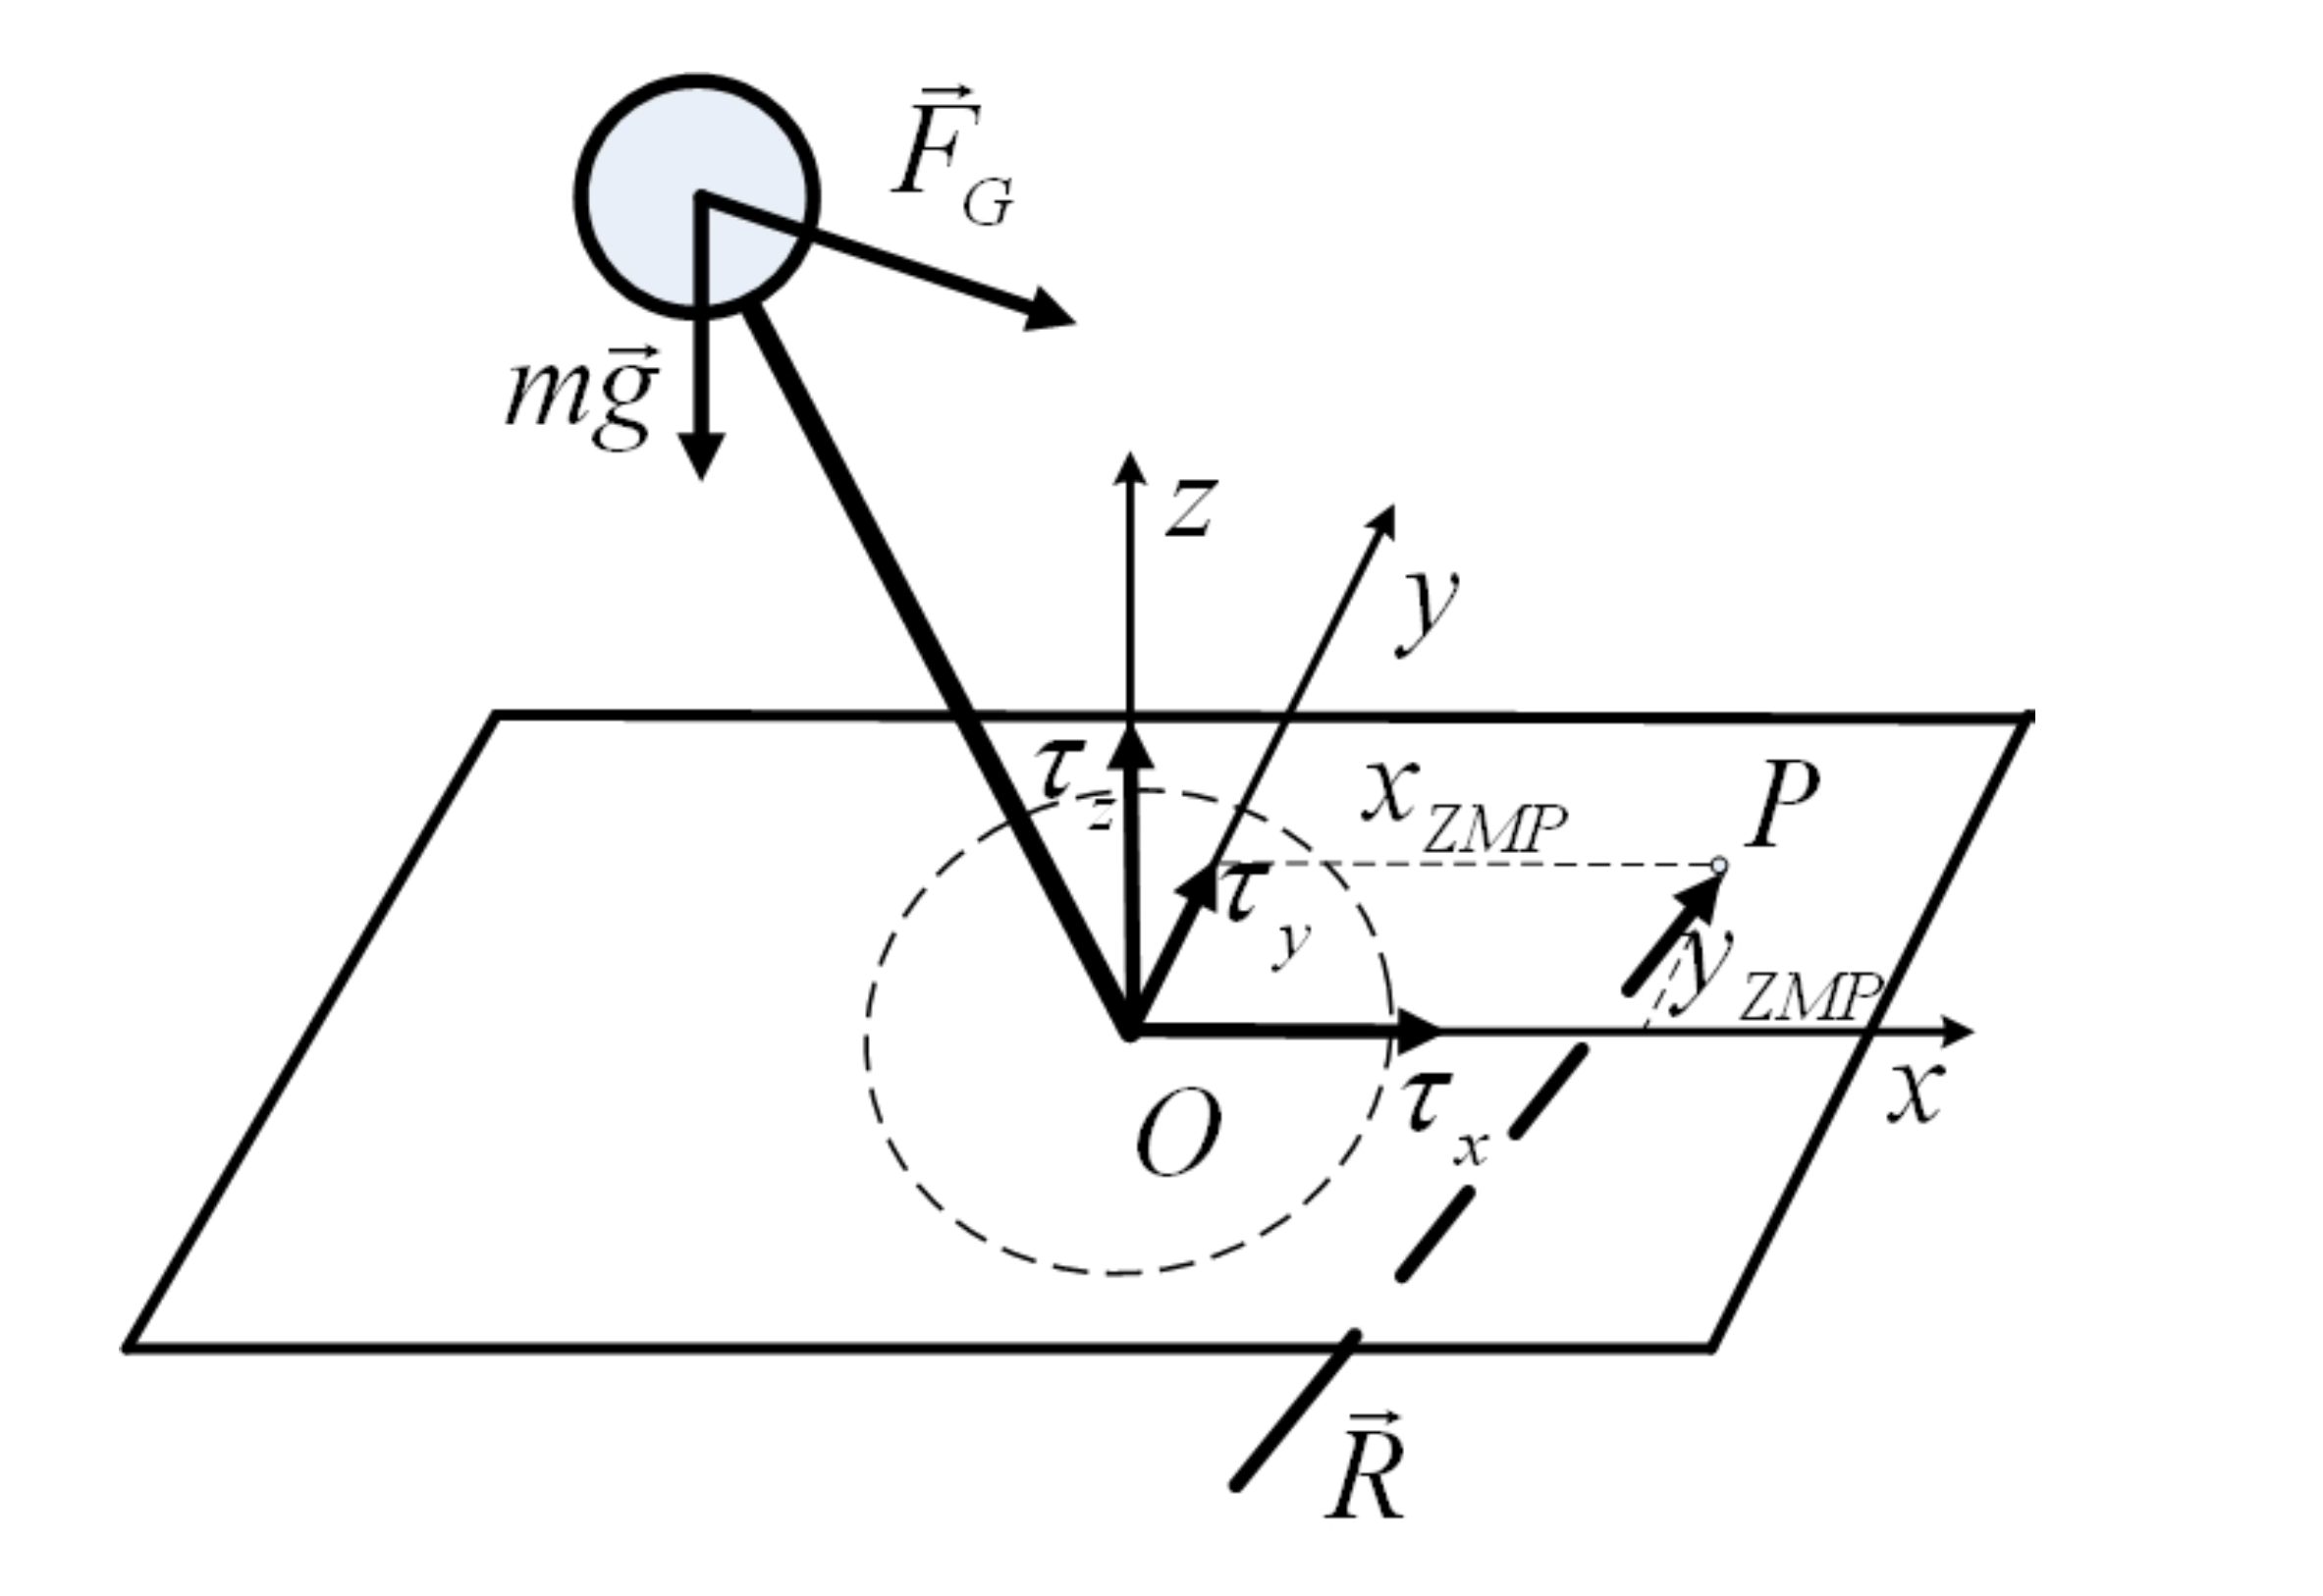
\includegraphics[scale=0.2]{3DLIPM.png}
\caption{3D Linear Inverted Pendulum with a contact polygon \protect\cite{Kaynov2008} }
\label{fig:3DLIPM}
\end{figure}

Inertial $\overrightarrow{F_G}$ and gravity $m\overrightarrow{g}$ froces act on the point mass located in the CoG of the humanoid robot. The contact of the pendulum with the ground produces a reaction force $\overrightarrow{R}$ and reaction moment $\overrightarrow{M_P}$ at point $P$. For any other point of the support polygon (taking point 0 as origin), the moment $M_0=[\tau_x, \tau_y, \tau_z]^T$ produced by the ground reaction force $\overrightarrow{R}$ is represented: 
\begin{equation}
M_0 = M_P + \overrightarrow{0P} \times \overrightarrow{R}
\label{eq:M0}
\end{equation}

If it is considered point P to be the ZMP of the system, then from the interpretation of the ZMP presented above $M_P = 0$. In this case we can denote vector $\overrightarrow{OP} = [x_{ZMP}, y_{ZMP}, z_{ZMP}]^T$ and eq. \eqref{eq:M0} gives the following equation:
\begin{equation}
\begin{pmatrix}
\tau_x \\
\tau_y \\
\tau_z 
\end{pmatrix} 
=
\begin{pmatrix}
x_{ZMP} \\
y_{ZMP} \\
z_{ZMP}
\end{pmatrix}
\times \overrightarrow{R}
\label{eq:1}
\end{equation}

From the other side, applying Newton’s law of mechanics to system in Figure \ref{fig:3DLIPM}:
\begin{equation}
m \overrightarrow{a_G} = \overrightarrow{R} - m\overrightarrow{g}
\label{eq:newton}
\end{equation}

where $\overrightarrow{a_G} = [\ddot{x}, \ddot{y}, \ddot{z}]^T$ is the acceleration of the CoG. From equation \eqref{eq:newton} it is obtained:
\begin{equation}
\overrightarrow{R} = m 
\begin{pmatrix}
\ddot{x} \\
\ddot{y} \\
\ddot{z} + g
\end{pmatrix}
\label{eq:2}
\end{equation}

Substituting equation \eqref{eq:2} into the equation of balance of moments \eqref{eq:1} it is obtained:
\begin{equation}
\begin{pmatrix}
\tau_x \\
\tau_y \\
\tau_z 
\end{pmatrix} 
= m
\begin{pmatrix}
x_{ZMP} \\
y_{ZMP} \\
z_{ZMP}
\end{pmatrix}
\times
\begin{pmatrix}
\ddot{x} \\
\ddot{y} \\
\ddot{z} + g
\end{pmatrix}
\end{equation}

After a cross product and taking into account that $z_{zmp} = 0$, because the ZMP lies into the ground:
\begin{equation}
\begin{pmatrix}
\tau_x \\
\tau_y \\
\tau_z 
\end{pmatrix} 
= m
\begin{pmatrix}
y_{ZMP}(\ddot{z}+g) \\
-x_{ZMP}(\ddot{z}+g) \\
x_{ZMP}\ddot{y}-y_{ZMP}\ddot{x}
\end{pmatrix}
\label{eq:3}
\end{equation}

From \eqref{eq:3}, it can be stated the ZMP position of the system:
\begin{equation}
x_{ZMP} = -\frac{\tau_y}{m(\ddot{z}+g)}
\label{eq:x}
\end{equation}
\begin{equation}
y_{ZMP} = \frac{\tau_x}{m(\ddot{z}+g)}
\label{eq:y}
\end{equation}

If it is supposed that the CoG always remains within the horizontal plain intersecting the $z$ axis in the point $z_c$ (one of the constraints of the 3D-LIPM model), then the vertical component of the CoG acceleration $\ddot{z}=0$. Then, finally, equations \eqref{eq:x} and \eqref{eq:y} are:
\begin{equation}
x_{ZMP} = -\frac{\tau_y}{mg}
\label{eq:xzmp}
\end{equation}
\begin{equation}
y_{ZMP} = \frac{\tau_x}{mg}
\label{eq:yzmp}
\end{equation}

When the ankle joint is displaced from the ground as in Figure \ref{fig:zmp_altura}, ZMP equations take the form:

\begin{equation}
x_{ZMP} = -\frac{\tau_y+hF_x}{mg}
\label{eq:xzmp}
\end{equation}
\begin{equation}
y_{ZMP} = \frac{\tau_x+hFy}{mg}
\label{eq:yzmp}
\end{equation}

where $h$ is the distance between the ground and the measuring point, i.e, the height of the sole. 
These are the \textit{ZMP equations}, without forgetting it was considered before that lateral accelerations of the COG $\ddot{x}=0$ and $\ddot{y}=0$. One can see that moments $\tau_x$ and $\tau_y$ in $x$ and $y$ directions respectively affect the ZMP position of the mecanism and it can loose balance because of their change.

\begin{figure}[!hbt]
\centering
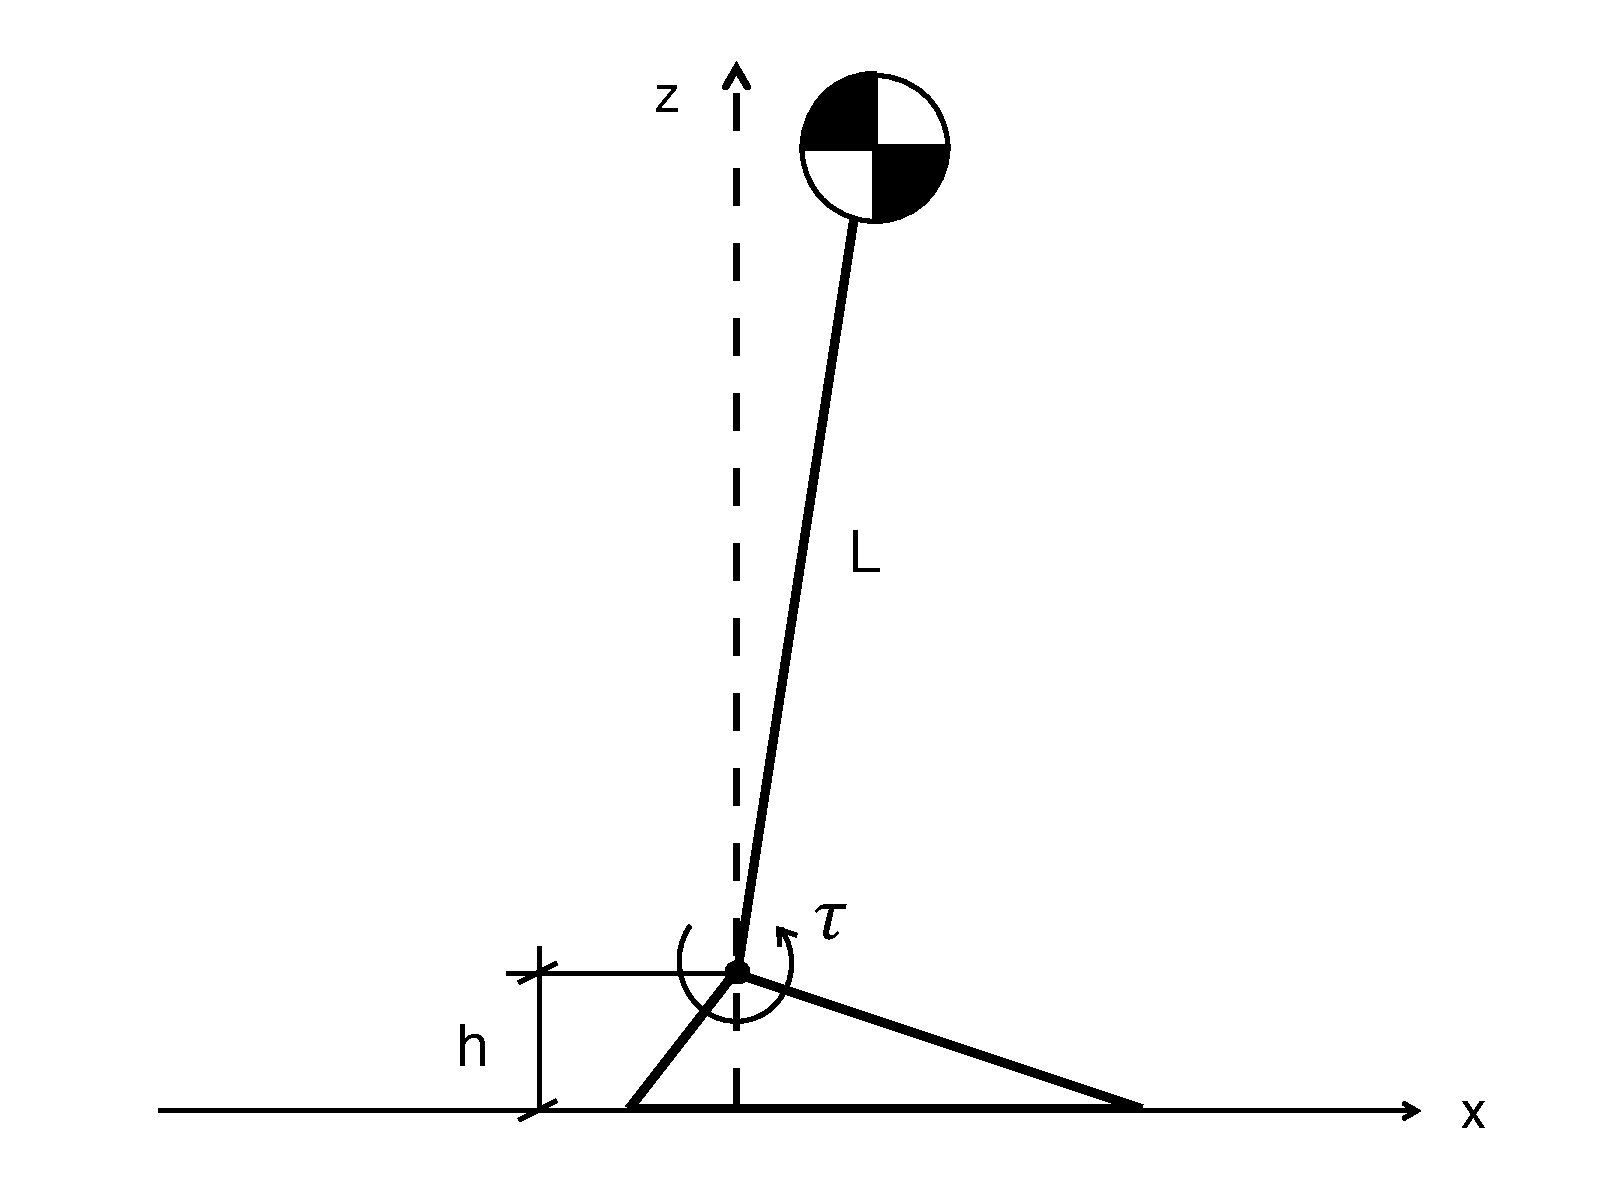
\includegraphics[scale=0.3]{alturaZMP.pdf}
\caption{Model for ZMP computation using F/T sensor measurements}
\label{fig:zmp_altura}
\end{figure}

If we take into account these lateral accelerations of the COG, the ZMP can be expressed as a function of the acceleration of the CoG as:
\begin{equation}
x_{ZMP}=x_{COG}-\frac{z_c}{g}\ddot{x}_{COG}
\end{equation}
\begin{equation}
y_{ZMP}=y_{COG}-\frac{z_c}{g}\ddot{y}_{COG}
\end{equation}

These equations can only be applied to compute ZMP in single-support phase. In the case of the double-support phase, it is necessary to calculate the weighted average of the sensor measurements form both feet as recommended in \cite[pp. 82-83]{Kaj2005}. Therefore, the resulting equations for ZMP in double-support phase are:

\begin{equation}
x_{ZMP} = -\frac{x_{ZMP}^{R} \cdot F_{z}^{R} + x_{ZMP}^{L} \cdot F_{y}^{L}}{F_{z}^{R}+F_{z}^{L}}
\end{equation}
\begin{equation}
y_{ZMP} = \frac{y_{ZMP}^{R} \cdot F_{z}^{R} + y_{ZMP}^{L} \cdot F_{z}^{L}}{F_{z}^{R}+F_{z}^{L}}
\end{equation}
where the upper index $R$ represents the right foot and $L$ the left one.

\subsection{ZMP areas.}
As mentioned before, ZMP is a point in the sole which depends on the forces and moments applied to the robot. Therefore, depending on the magnitude of that forces, ZMP will change and it becomes a dynamic parameter. As suggested in \cite{Vuk2007}, three regions are defined depending on the position of the ZMP as one can see in Fig. \ref{fig:zonas}.
In the balanced area (safe region), the control action will not actuate. In the nearly critical region, the control action will actuate as a secondary solution. This may be the case of a walking task. As humans do, the robot may use its arms in order to reduce the zero-moment point position closer to the safe region. Finally, in the critical region, the stabilizer will actually disconnect the ongoing task and actuate on the full body. Even if this region is still stable, the balance may be easily lost. 


\begin{figure}[!hbt]
\centering
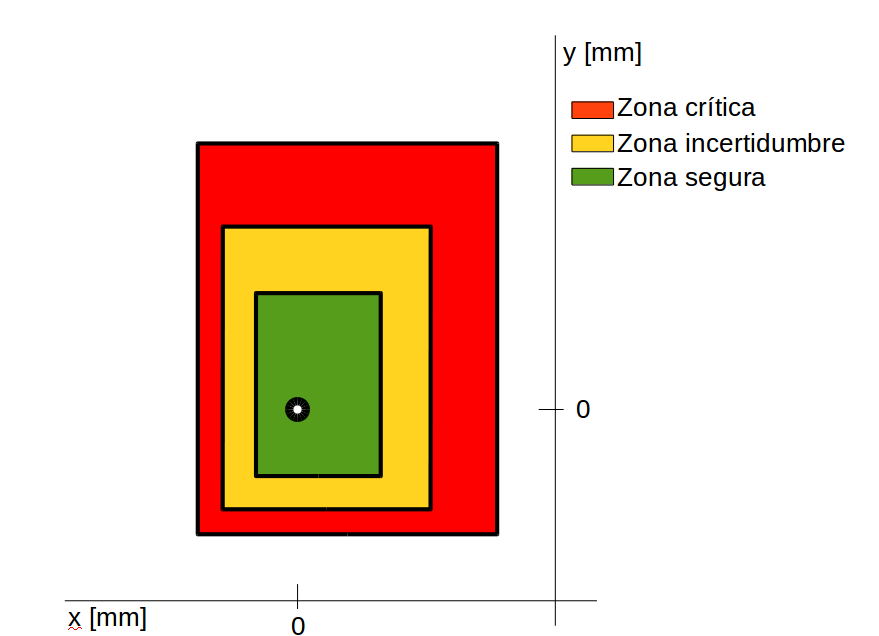
\includegraphics[scale=0.3]{zonas}
\caption{ZMP stability regions in single-support.}
\label{fig:zonas}
\end{figure}



%\section{Biped modeling}
%Humanoid robots have a very complex dynamics because of their complex mechanical configuration and they require a high computational cost. Figure ??? represents a simplified mechanical configuration of a typical humanoid robot. As one can see, the high number of DOFs due to the precise knowledge of robot dynamics including, mass, location of the centre of mass and moments of inertia of each link, make stable biped locomotion very complex. Thus, different simplified models of the mechanics have been developed. These methods use limited knowledge of the dynamics and the humanoid is usually represented by a planar inverted pendulum with the base representing the ankle joint and, in case of 3D locomotion, the Three-Dimensional Inverted Pendulum Mode (3D-LIPM) \cite{Kaj2001}.
